\documentclass[lualatex,aspectratio=169]{beamer}
\usepackage[T1]{fontenc}
\usepackage{luatexja}
\usepackage[deluxe]{luatexja-preset} 
\usepackage{amsmath}
\usepackage{tikz}
\usepackage{listings}
\lstset{
  basicstyle=\footnotesize\ttfamily,
  keywordstyle=\color{blue},
  language=[LaTeX]TeX,
  breaklines=true,
  showstringspaces=false,
}
\setmainjfont{Hiragino Kaku Gothic ProN}

\usetheme[progressbar=none]{metropolis}

\usepackage{xcolor}
\definecolor{hf-orange}{HTML}{FFA700}
\definecolor{hf-orange-dark}{HTML}{FF882B}
\definecolor{hf-blue}{HTML}{4884DA}
\definecolor{hf-blue-dark}{HTML}{4D6BD5}
\definecolor{hf-orange-gradient-left}{HTML}{FF882B}
\definecolor{hf-orange-gradient-right}{HTML}{FFE721}
\definecolor{hf-blue-gradient-left}{HTML}{48D2E6}
\definecolor{hf-blue-gradient-right}{HTML}{4D6BD5}

\setbeamertemplate{footline}{%
  \begin{tikzpicture}[remember picture, overlay]
    % left half of the bar
    \shade[left color=hf-orange-gradient-left, right color=hf-orange-gradient-right]
      (current page.south west) rectangle ([yshift=0.5mm]current page.south);

    % right half of the bar
    \shade[left color=hf-blue-gradient-left, right color=hf-blue-gradient-right]
      (current page.south) rectangle ([yshift=0.5mm]current page.south east);

    % slide number
    \node[
      anchor=east,
      xshift=-5mm,
      yshift=5mm,
      font=\sffamily\color{mDarkTeal}
    ]
    at (current page.south east)
    {\insertframenumber};
  \end{tikzpicture}%
}

\setbeamertemplate{title separator}{
  
\begin{tikzpicture}
    % Left half of the bar
    \shade[left color=hf-orange-gradient-left, right color=hf-orange-gradient-right]
      (0,0) rectangle (0.5\textwidth, 0.25mm);
    % Right half of the bar
    \shade[left color=hf-blue-gradient-left, right color=hf-blue-gradient-right]
      (0.5\textwidth,0) rectangle (\textwidth, 0.25mm);
  \end{tikzpicture}
  \vskip1em % Adds a little vertical space after the separator
}

\setbeamertemplate{section page}{
  \begin{center}
    \usebeamerfont{section title}
    \usebeamercolor[fg]{section title}
    \insertsection
    \par % Creates a new paragraph for spacing
    
\begin{tikzpicture}
      % Left half of the bar
      \shade[left color=hf-orange-gradient-left, right color=hf-orange-gradient-right]
        (0,0) rectangle (0.5\textwidth, 0.25mm);
      % Right half of the bar
      \shade[left color=hf-blue-gradient-left, right color=hf-blue-gradient-right]
        (0.5\textwidth,0) rectangle (\textwidth, 0.25mm);
    \end{tikzpicture}
  \end{center}
}

\setbeamercolor{frametitle}{fg=mDarkTeal, bg=black!2}
\setbeamertemplate{frametitle}{
  \nointerlineskip%
  \begin{tikzpicture}
    % use the full paper width and a height of 5ex
    \useasboundingbox (0,0) rectangle (\paperwidth, 5ex);

    % background for the entire header
    \fill[black!2] (0,0) rectangle (\paperwidth, 5ex);

    % thin gradient bar on the left (top to bottom)
    \shade[top color=hf-orange-gradient-left, bottom color=hf-orange-gradient-right] (0,0) rectangle (1.5mm, 5ex);

    % frame title text (mDarkTeal on black!2)
    \node[
      anchor=west,      % align text to the left
      inner xsep=1em,     % add padding between bar and text
      text=mDarkTeal
    ] at (2mm, 2.5ex) { % position the node
      \usebeamerfont{frametitle}\insertframetitle
    };
  \end{tikzpicture}%
}

\title{IT+$\alpha$}
\subtitle{IT以外の分野への熱心も生き残るITキャリア}
\author{tarek(タレク)}
\institute{株式会社Helpfeel}
\date{}

\begin{document}

\begin{frame}[plain]
  \titlepage
\end{frame}

% \begin{frame}[t]{目次}
%   \tableofcontents
% \end{frame}

% \section{自己紹介}

\begin{frame}[t]{自己紹介 / LTの内容}
    \begin{figure}
        \begin{overprint}
            \onslide<1>\begin{center}
\includegraphics[width=0.8\linewidth]{./img/intro_0.pdf}\end{center}
            \onslide<2>\begin{center}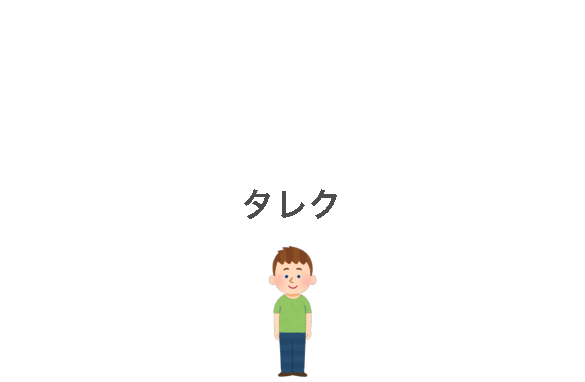
\includegraphics[width=0.8\linewidth]{./img/intro_1.pdf}\end{center}
            \onslide<3>\begin{center}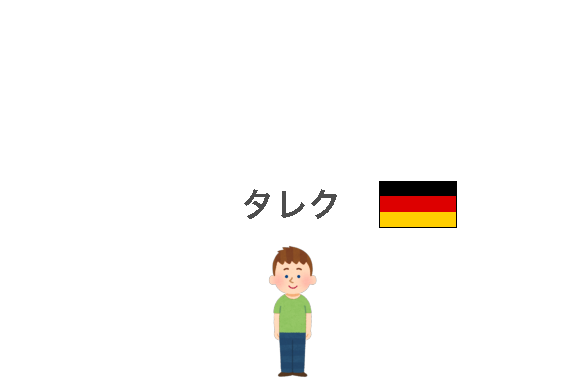
\includegraphics[width=0.8\linewidth]{./img/intro_1-1.pdf}\end{center}
            \onslide<4>\begin{center}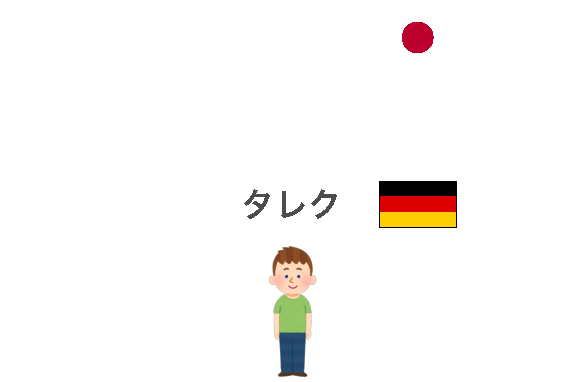
\includegraphics[width=0.8\linewidth]{./img/intro_1-2.pdf}\end{center}
            \onslide<5>\begin{center}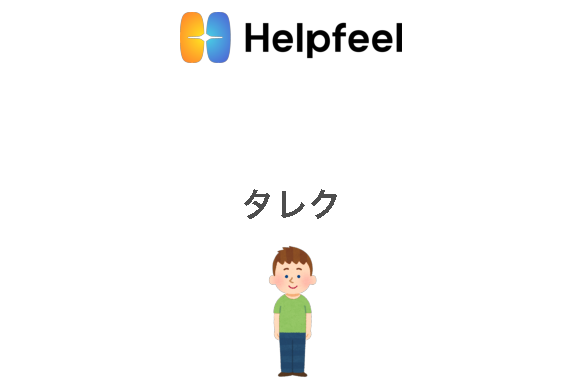
\includegraphics[width=0.8\linewidth]{./img/intro_2.pdf}\end{center}
            \onslide<6>\begin{center}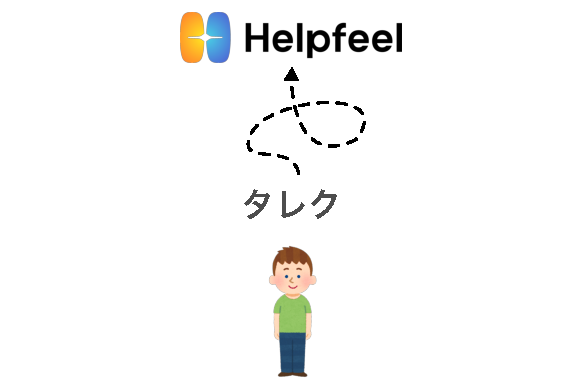
\includegraphics[width=0.8\linewidth]{./img/intro_3.pdf}\end{center}
        \end{overprint}
    \end{figure}
\end{frame}

\begin{frame}[t]
    \frametitle<1>{ITでいいのか?と悩んで...}
    \frametitle<2-6>{ITを選んでしまって...}
    \frametitle<7>{でもたくさんの「+$\alpha$」を楽しめています}
    \begin{figure}
        \begin{overprint}
            \onslide<1>\begin{center}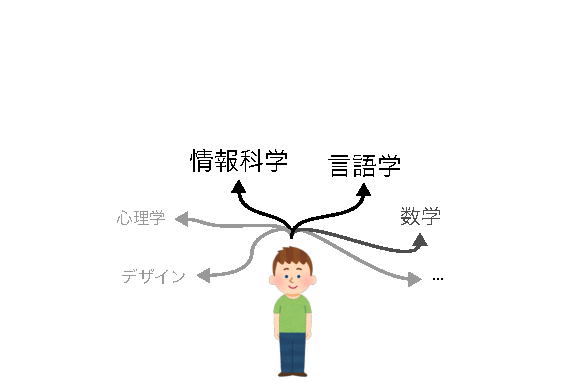
\includegraphics[width=0.8\linewidth]{./img/intro_4.pdf}\end{center}

            \onslide<2>\begin{center}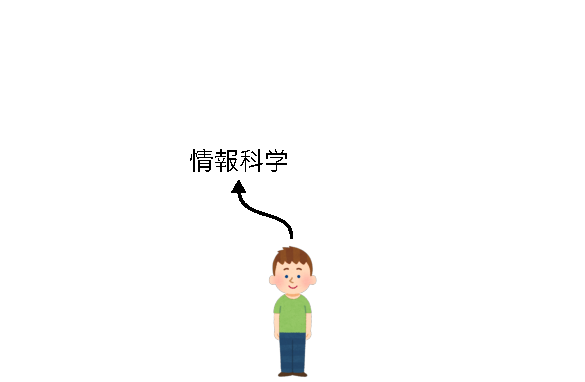
\includegraphics[width=0.8\linewidth]{./img/intro_5.pdf}\end{center}
            \onslide<3>\begin{center}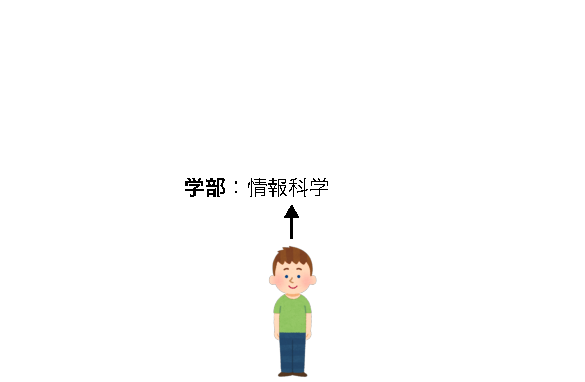
\includegraphics[width=0.8\linewidth]{./img/intro_6.pdf}\end{center}
            \onslide<4>\begin{center}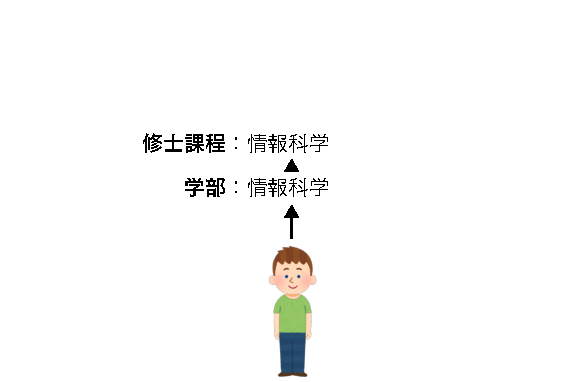
\includegraphics[width=0.8\linewidth]{./img/intro_7.pdf}\end{center}
            \onslide<5>\begin{center}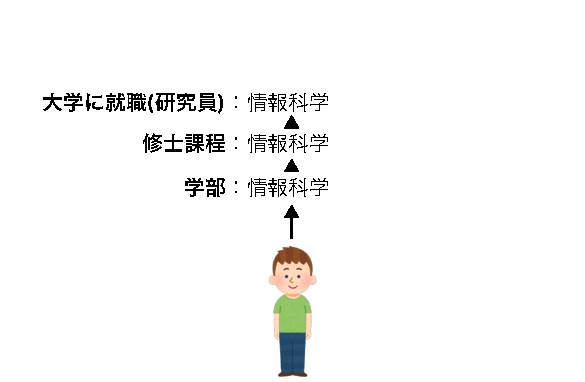
\includegraphics[width=0.8\linewidth]{./img/intro_8.pdf}\end{center}
            \onslide<6>\begin{center}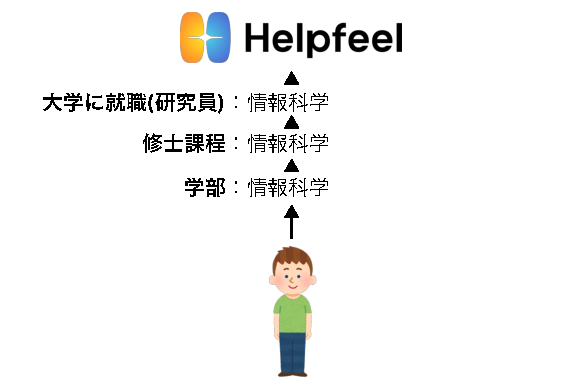
\includegraphics[width=0.8\linewidth]{./img/intro_9.pdf}\end{center}

            \onslide<7>\begin{center}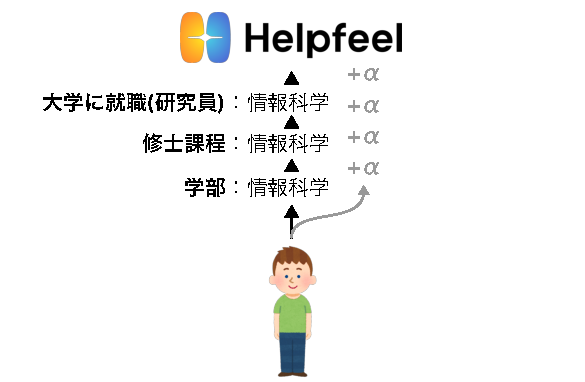
\includegraphics[width=0.8\linewidth]{./img/intro_10.pdf}\end{center}
        \end{overprint}
    \end{figure}
\end{frame}

\begin{frame}[t]{LTの内容 / メッセージ}
    事例として
    \begin{itemize}
        \item \textbf{タレクの\,+$\mathbf{\alpha}$エピソード3選}
        \item {\color{gray}おまけ:それぞれにちょっとした学び}
    \end{itemize}
    \vspace{2em}
    $\rightarrow$~「ITキャリアを歩みながらIT以外の分野も楽しめます!」
\end{frame}

% \begin{frame}[t]{+$\alpha$のエピソード}
%     \begin{enumerate}
%         \item 言語学習SNSで他人のアカウントを乗っ取って、\\課金せずにプレミアムアカウントを手に入れたとき
%         \item 文字も読めない言語を研究対象としたとき
%         \item 100万人以上の論文をコピペして自分のものとして公開したとき
%     \end{enumerate}
% \end{frame}

\section{+$\alpha$のエピソード その1}

\section{日本語学習でもITセキュリティを考えて得した}
% \section{言語学習SNSの脆弱性}
% \section{言語学習SNSで他人のアカウントを乗っ取って、\\課金せずにプレミアムアカウントを手に入れたとき}

\begin{frame}[t]{+$\alpha$のエピソード その1}
    % 言語学習SNS(Lang-8)の脆弱性を報告したエピソード
    言語学習SNSの脆弱性を報告して1年間のプレミアムアカウントを手に入れた
    \begin{figure}
        \onslide<2->\begin{center}
\includegraphics[width=0.8\linewidth]{./img/lang8_1.png}\end{center}
        \onslide<3->\begin{center}
\includegraphics[width=0.8\linewidth]{./img/lang8_2.png}\end{center}
    \end{figure}
    \onslide<4>\textbf{学び:}趣味でも本業の遊び心を忘れず\\
 	\onslide<4>\textbf{学び:}ユーザからの入力をちゃんと前処理しましょう
\end{frame}

\section{+$\alpha$のエピソード その2}

\section{機械学習ゼミを行なってキリル文字を読めるようになった}
% \section{キリル文字論文からの情報抽出}
% \section{文字も読めない言語を研究対象としたとき}

\begin{frame}[t]{+$\alpha$のエピソード その2}
    ローマ字以外の言語で書いてある学術論文からの情報抽出
    \begin{figure}
        \begin{overprint}
            \onslide<2>\begin{center}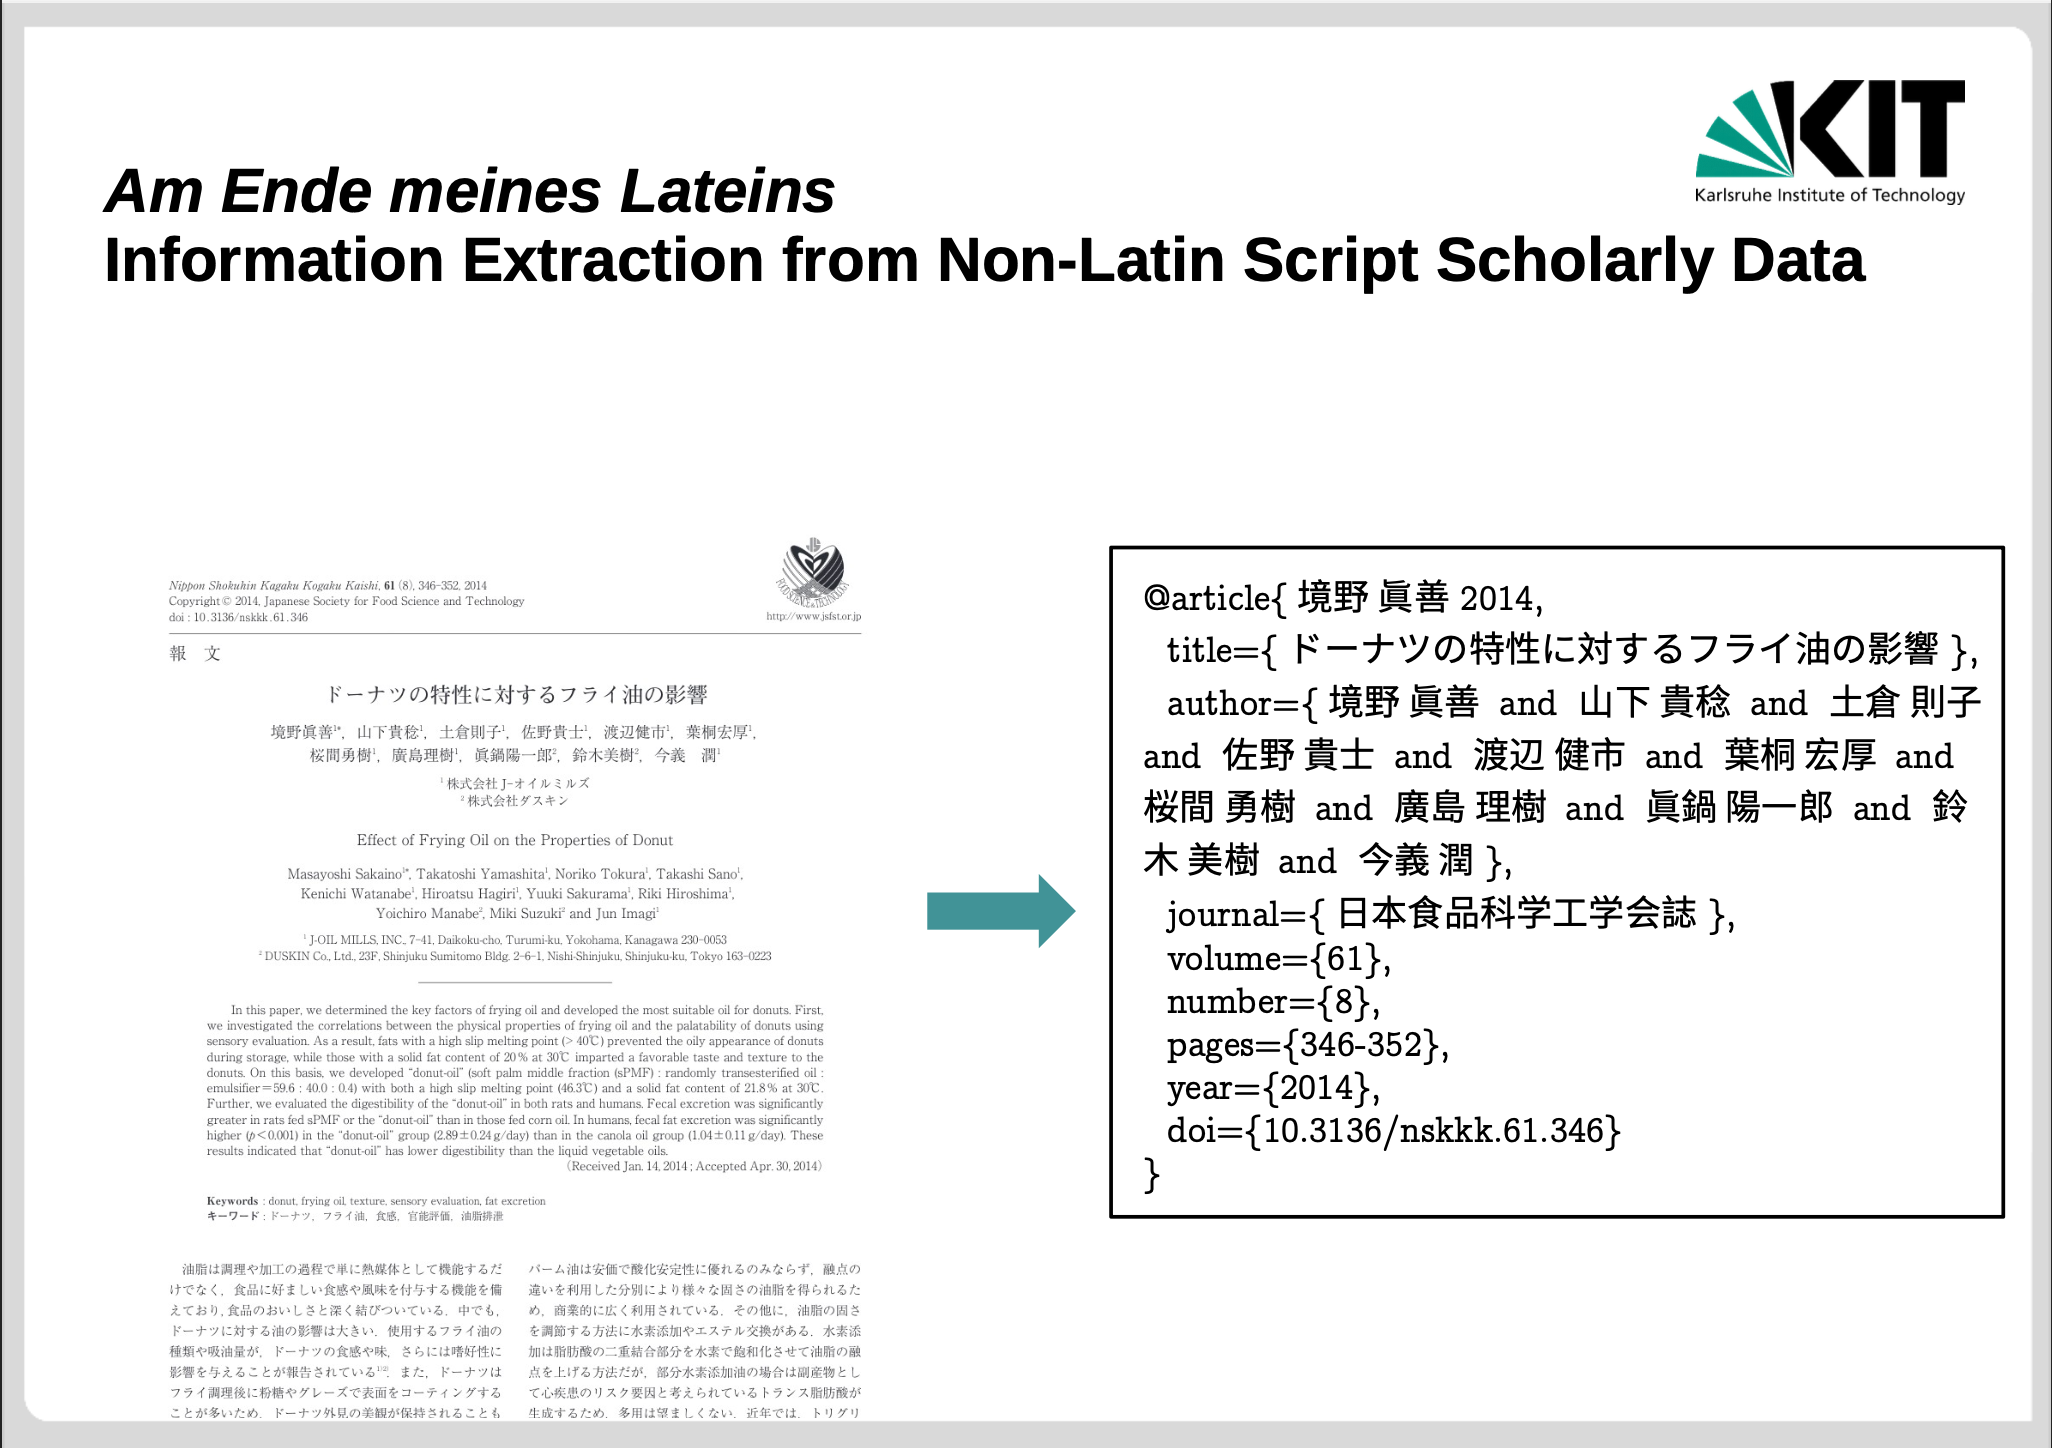
\includegraphics[height=0.45\textheight]{./img/cyr_1.png}\end{center}
            \onslide<3>\begin{center}
\includegraphics[height=0.45\textheight]{./img/cyr_2.png}\end{center}
            \onslide<4>\begin{center}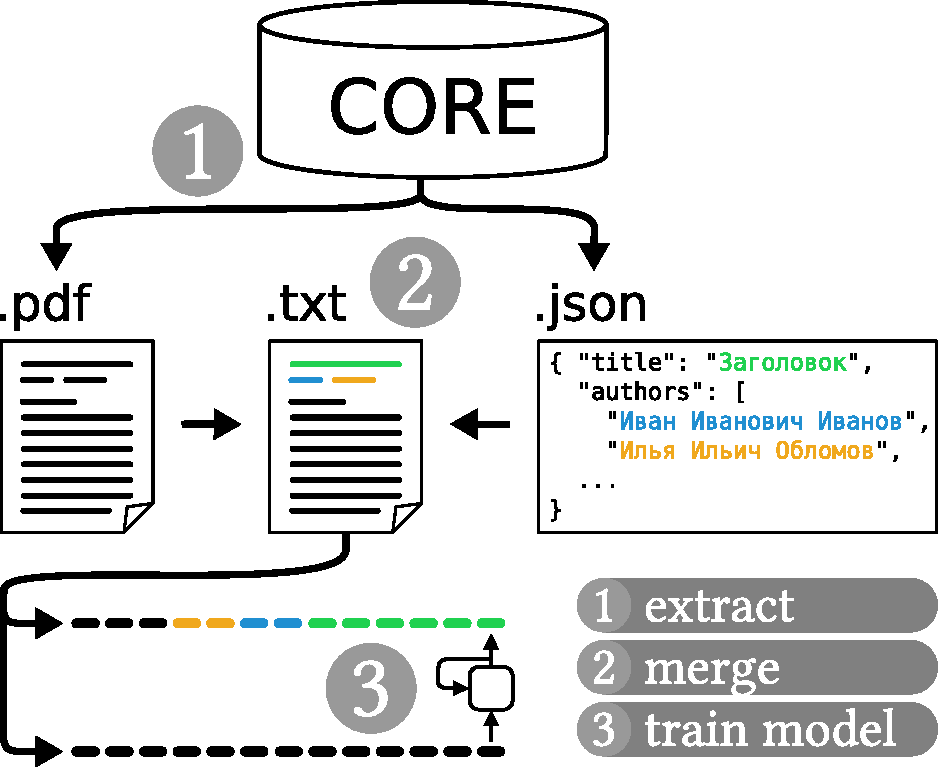
\includegraphics[height=0.45\textheight]{./img/cyr_ppr_1_2.pdf}\end{center}
            \onslide<5>\begin{center}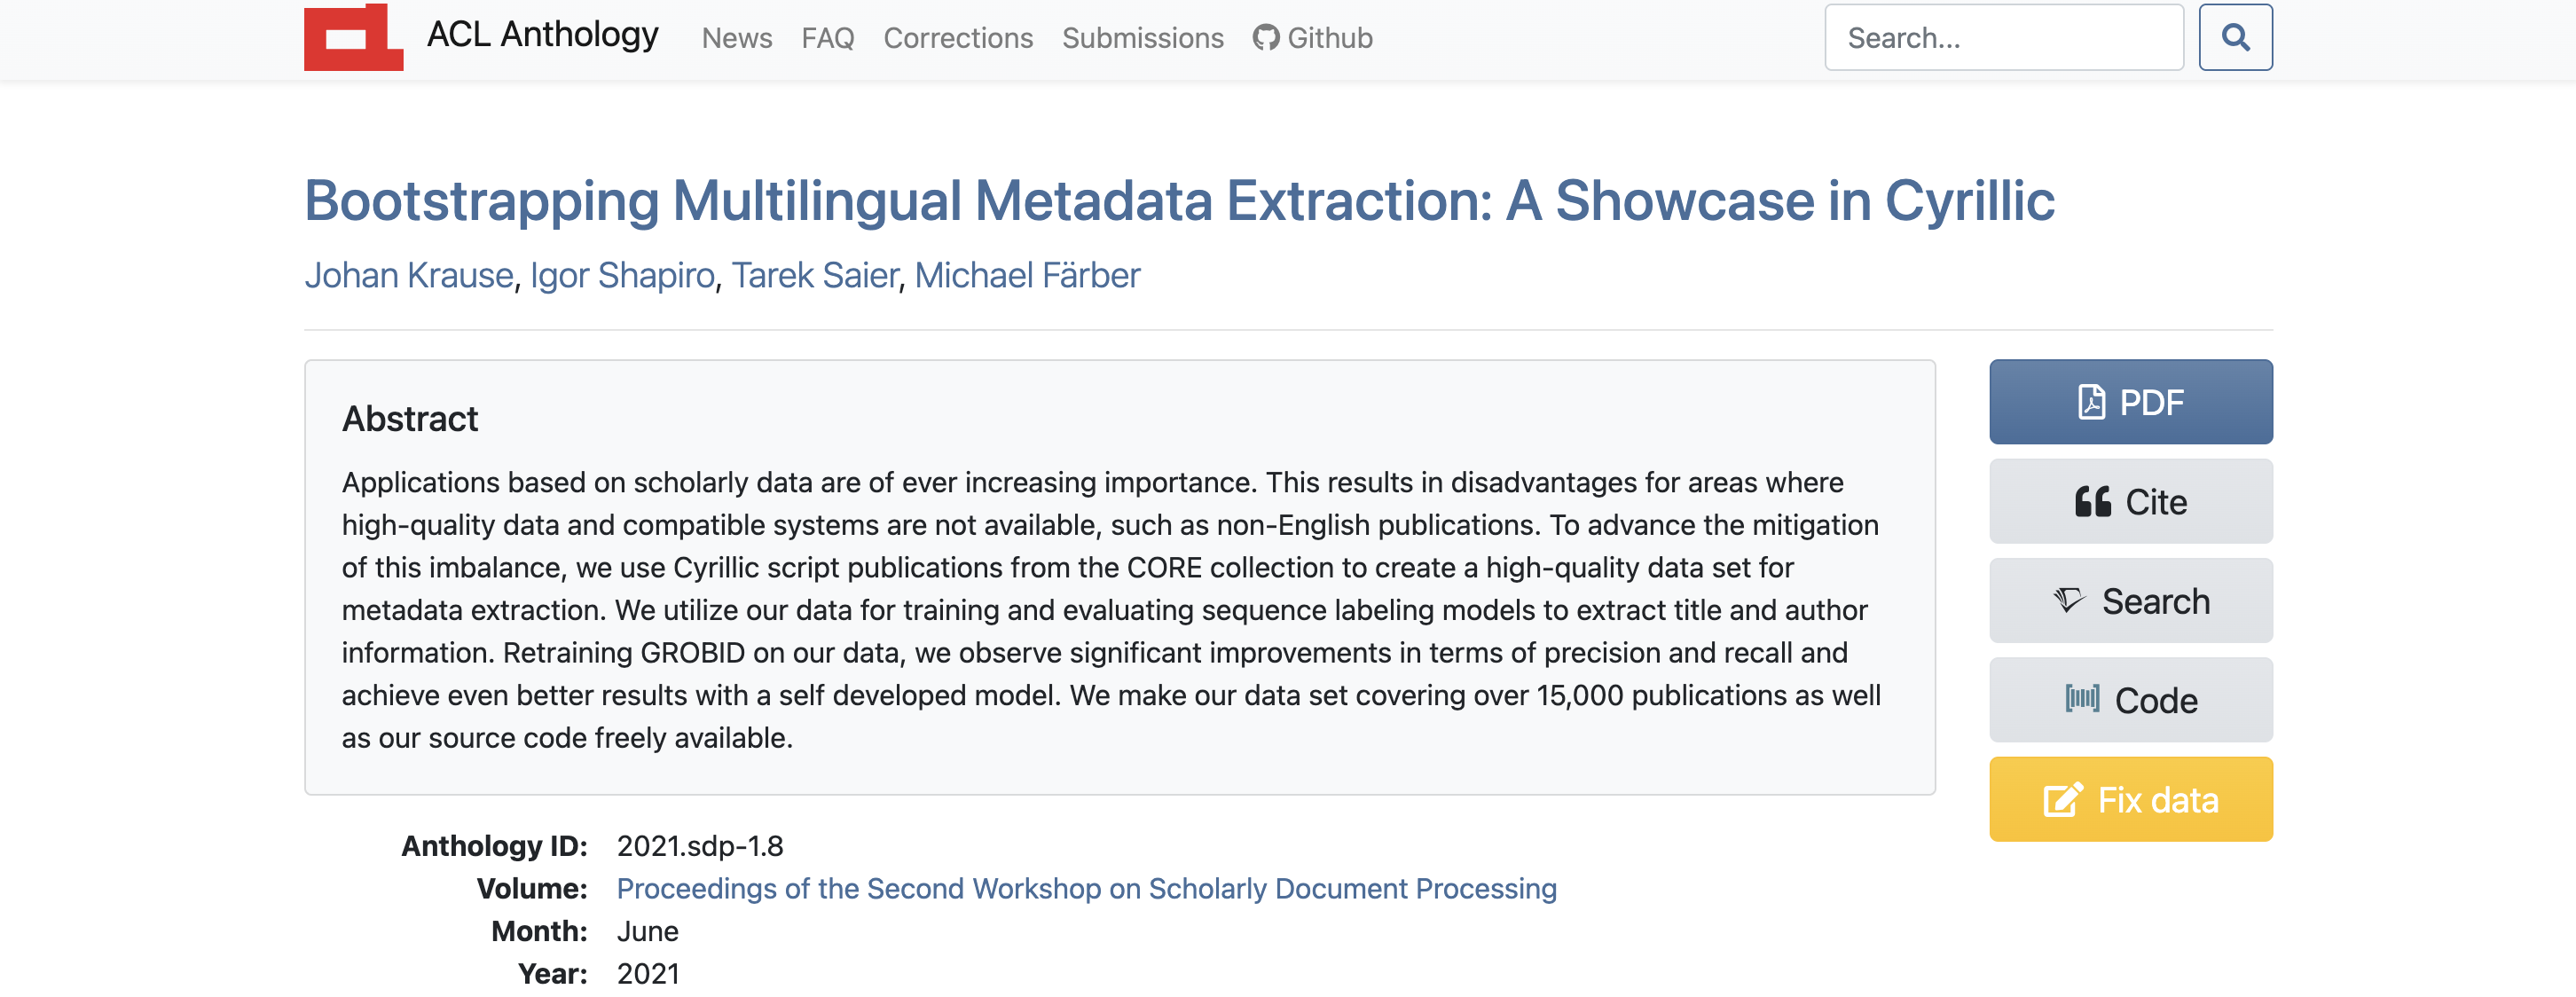
\includegraphics[height=0.45\textheight]{./img/cyr_ppr_1_1.png}\end{center}
            \onslide<6>\begin{center}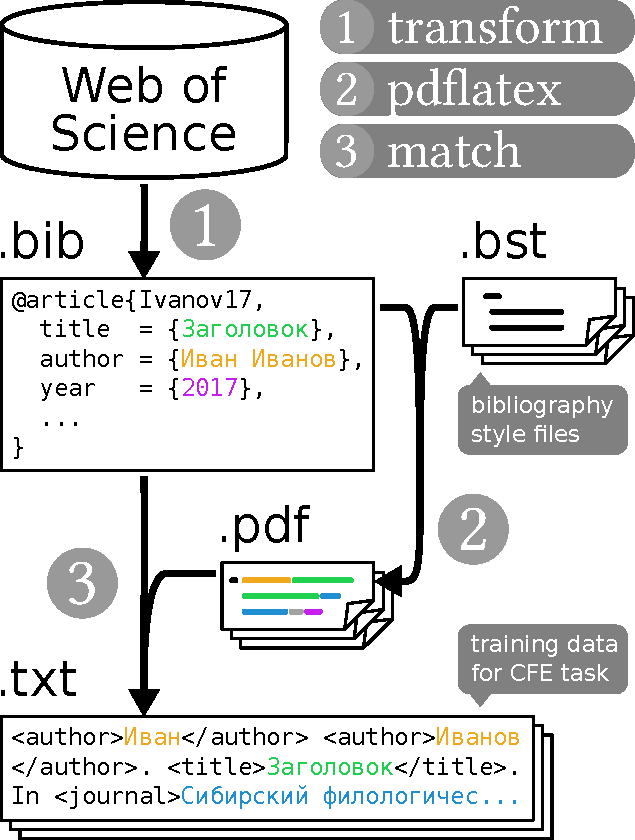
\includegraphics[height=0.45\textheight]{./img/cyr_ppr_2_2.pdf}\end{center}
            \onslide<7-8>\begin{center}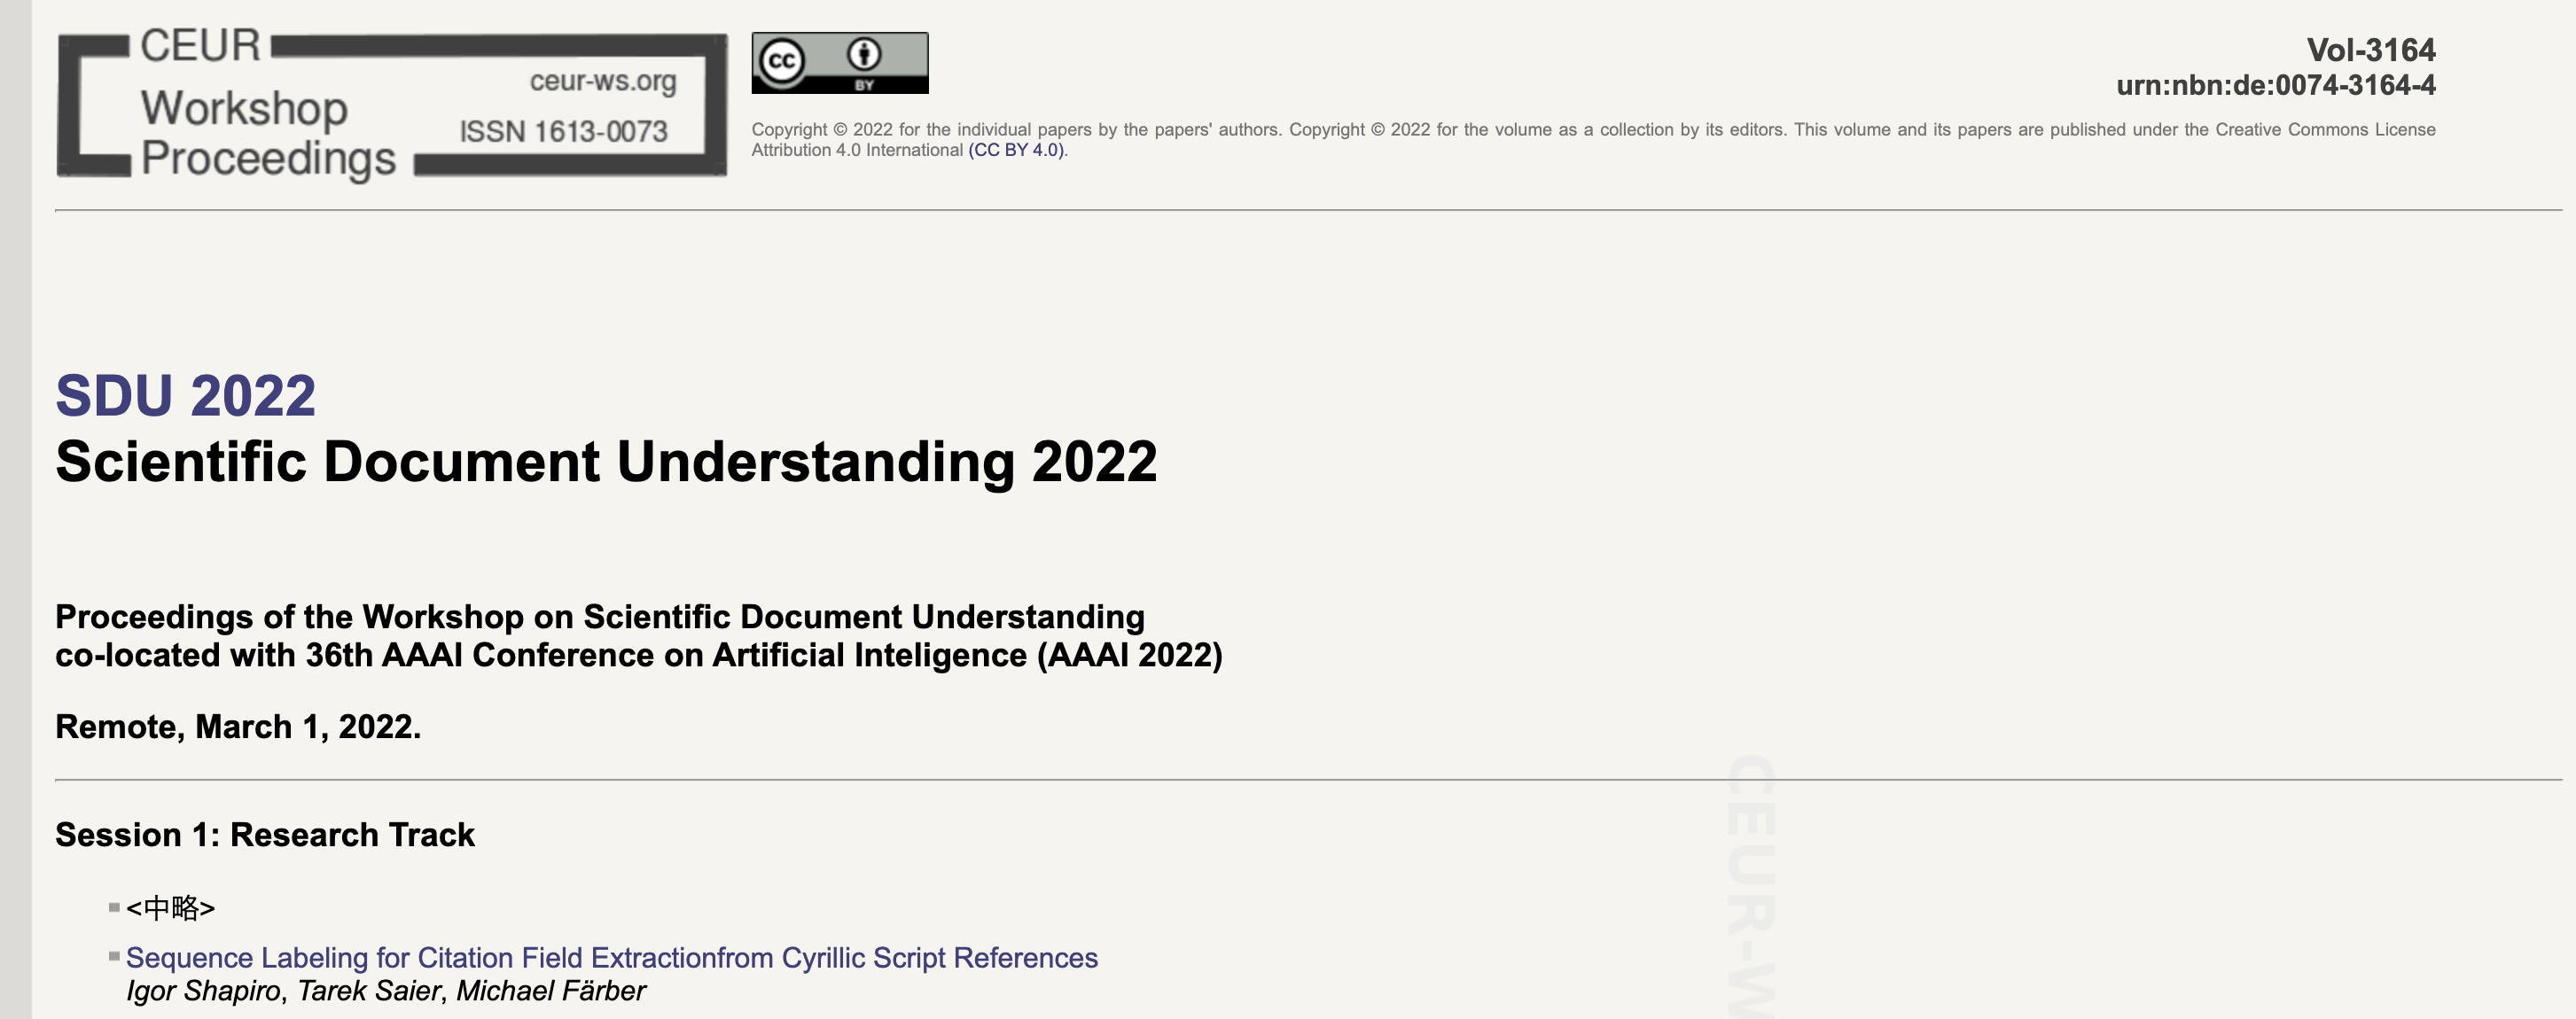
\includegraphics[height=0.45\textheight]{./img/cyr_ppr_2_1.png}\end{center}
            \onslide<9->\begin{center}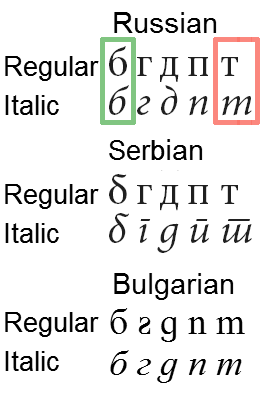
\includegraphics[height=0.4\textheight]{./img/cyr_italics_marked.png}\\{\tiny\url{https://en.wikipedia.org/wiki/File:Special_Cyrillics.png}}\end{center}
        \end{overprint}
    \end{figure}
    \onslide<8->\textbf{学び:}他人が得意を活かせる場を用意できたらやる気がでる\\
 	\onslide<8->\textbf{学び:}キリル文字のイタリック体は一部が完全に別の文字になる
\end{frame}

\section{+$\alpha$のエピソード その3}

\section{機械学習データセットを作って\LaTeX{}の理解が深まった}
% \section{論文の\TeX{}ソースから作ったデータセット}
% \section{100万人以上の論文をコピペして自分のものとして公開したとき}

\begin{frame}[t]{+$\alpha$のエピソード その3}
    100万本の論文の\LaTeX{}ソースからデータセットを作ってブチバズった話
    \begin{figure}
        \begin{overprint}
            \onslide<2>\begin{center}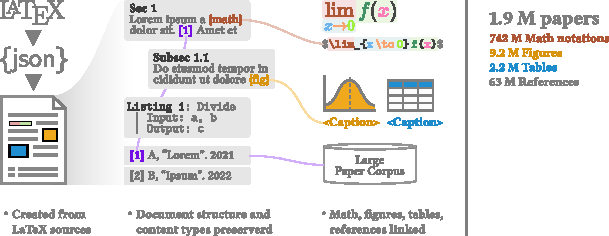
\includegraphics[height=0.45\textheight]{./img/unarxive_schema.pdf}\end{center}
            \onslide<3>\begin{center}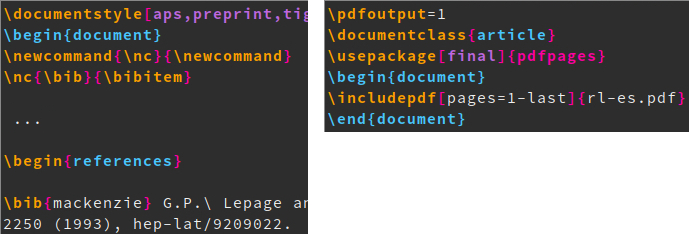
\includegraphics[height=0.45\textheight]{./img/weirdtex.png}\end{center}
            \onslide<4->\begin{center}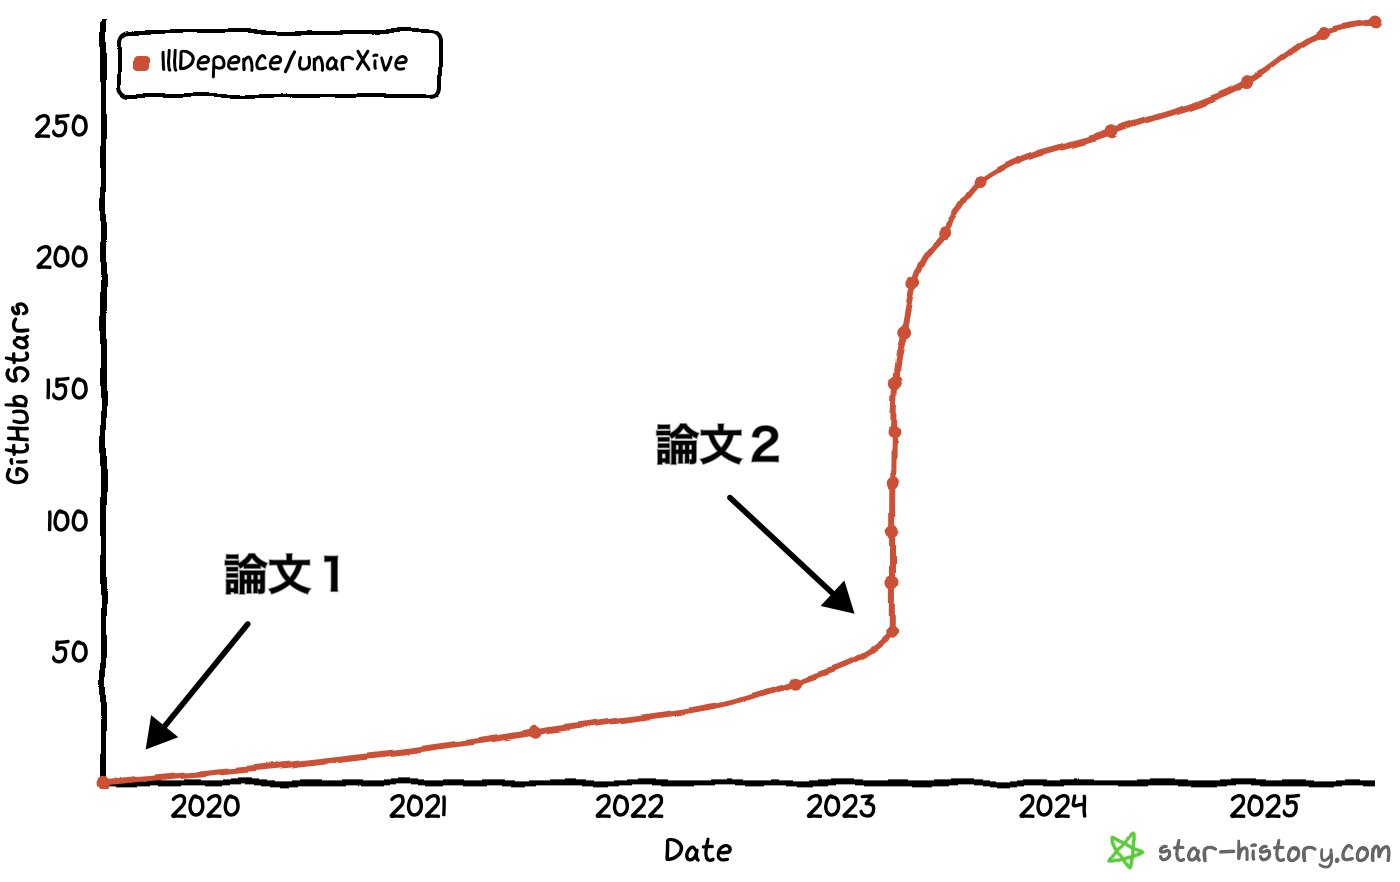
\includegraphics[height=0.45\textheight]{./img/unarxive_stars_annot.png}\end{center}
        \end{overprint}
    \end{figure}
    \onslide<5>\textbf{学び:}好きなものを仕事の対象にできたらやる気がでていいもの作れる\\
 	\onslide<5>\textbf{学び:}発信しつづけるのが大事
\end{frame}

\section{まとめ}

\begin{frame}[t]{IT+$\alpha$}
    \vspace{3em}
    \begin{center}
        {\Large ITキャリアを歩みながらIT以外の分野も楽しめます!}\\
        \vspace{0.5em}
        {\color{lightgray}tarekの言語・文字への熱心が生きていて元気です!}\\
        \vspace{1.5em}
        {\color{lightgray}---}\\
        \vspace{1.5em}
        {\color{lightgray}あなたの「+$\alpha$」は何でしょう?}
    \end{center}
\end{frame}

\begin{frame}[t]{ご清聴ありがとうございました}
    tarek(タレク)\\
    株式会社Helpfeel
    \begin{columns}
    \begin{column}{0.3\textwidth}
        \begin{center}
        \begin{figure}
        
\includegraphics[width=0.7\textwidth]{./img/qr_github.png}
        \end{figure}
        \footnotesize\texttt{github.com/IllDepence}
        \end{center}
    \end{column}
    \begin{column}{0.3\textwidth}
        \begin{center}
        \begin{figure}
        
\includegraphics[width=0.7\textwidth]{./img/qr_blog.png}
        \end{figure}
        \footnotesize\texttt{sirtetris.com}
        \end{center}
    \end{column}
    \begin{column}{0.3\textwidth}
        \begin{center}
        \begin{figure}
        
\includegraphics[width=0.7\textwidth]{./img/qr_slides.png}
        \end{figure}
        \footnotesize\texttt{スライド}
        \end{center}
    \end{column}
    \end{columns}
\end{frame}

\end{document}
